% !TeX spellcheck = en_US
%\documentclass{beamer}
\documentclass[handout]{beamer}
\usepackage[spanish]{babel}
\usepackage[utf8]{inputenc}
\usepackage{graphicx}
\usepackage{tcolorbox}
%\setbeamercolor{frametitle}{fg=white}
%\usefonttheme{structuresmallcapsserif}
%\setbeamertemplate{footline}[frame number]
%\setbeamerfont{footnote}{size=\tiny}

\usepackage{default}

\usepackage[backend = bibtex, style = verbose, sorting = none, autocite = footnote]{biblatex}
\addbibresource{references.bib}

\newcommand\blfootnote[1]
{%
	\begingroup
	\renewcommand\thefootnote{}\footnote{#1}%
	\addtocounter{footnote}{-1}%
	\endgroup
}
\newcommand{\fcite}[1]{\blfootnote{\cite{#1}}}

\usetheme{Berkeley}

\begin{document}
	\begin{frame}
		\centering
		%\color{white}
		\textsc{\Large Start-up and calibration of a 2277 ThermoMetric calorimeter}
		\\
		\vspace{5cm}
		\raggedleft \textbf{Presented by:} Juan Barbosa\\
		\raggedleft \textbf{Directed by:} Edgar Vargas, Dr. Sc.\\
		\raggedleft \textbf{Group of Thermodynamics of Solutions}
	\end{frame}

\begin{frame}{Contents}
	\tableofcontents
\end{frame}

\section{Introduction}
\begin{frame}{Introduction}
	\begin{table}[h]
		\centering
		\begin{tabular}{ccc}
			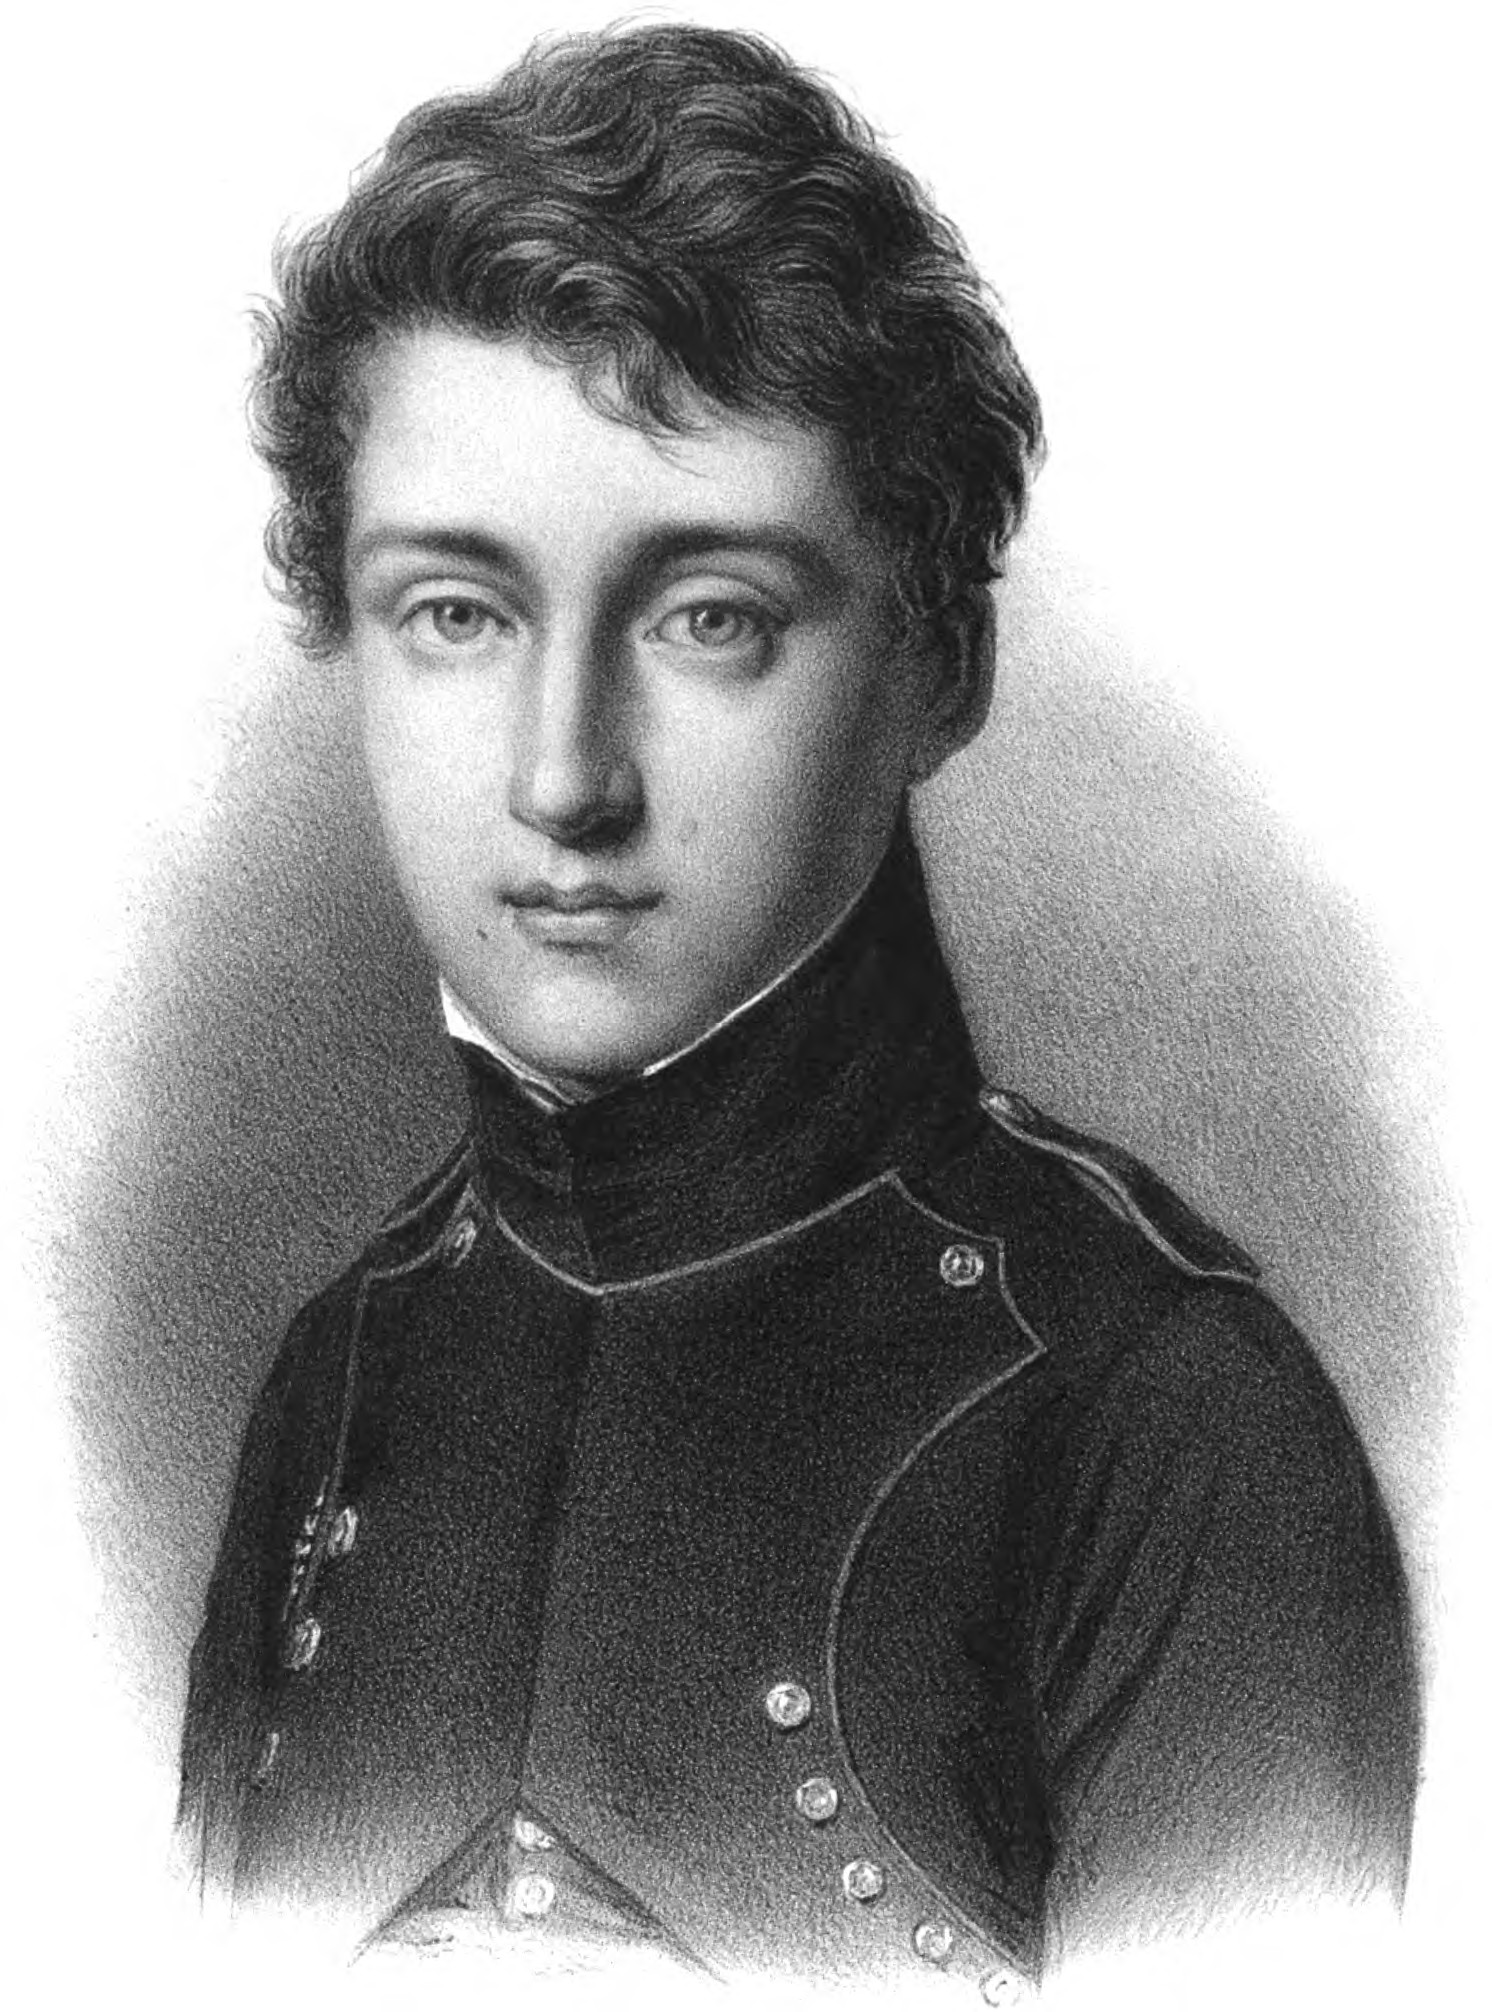
\includegraphics[width=0.25\linewidth]{sources/carnot} & 
			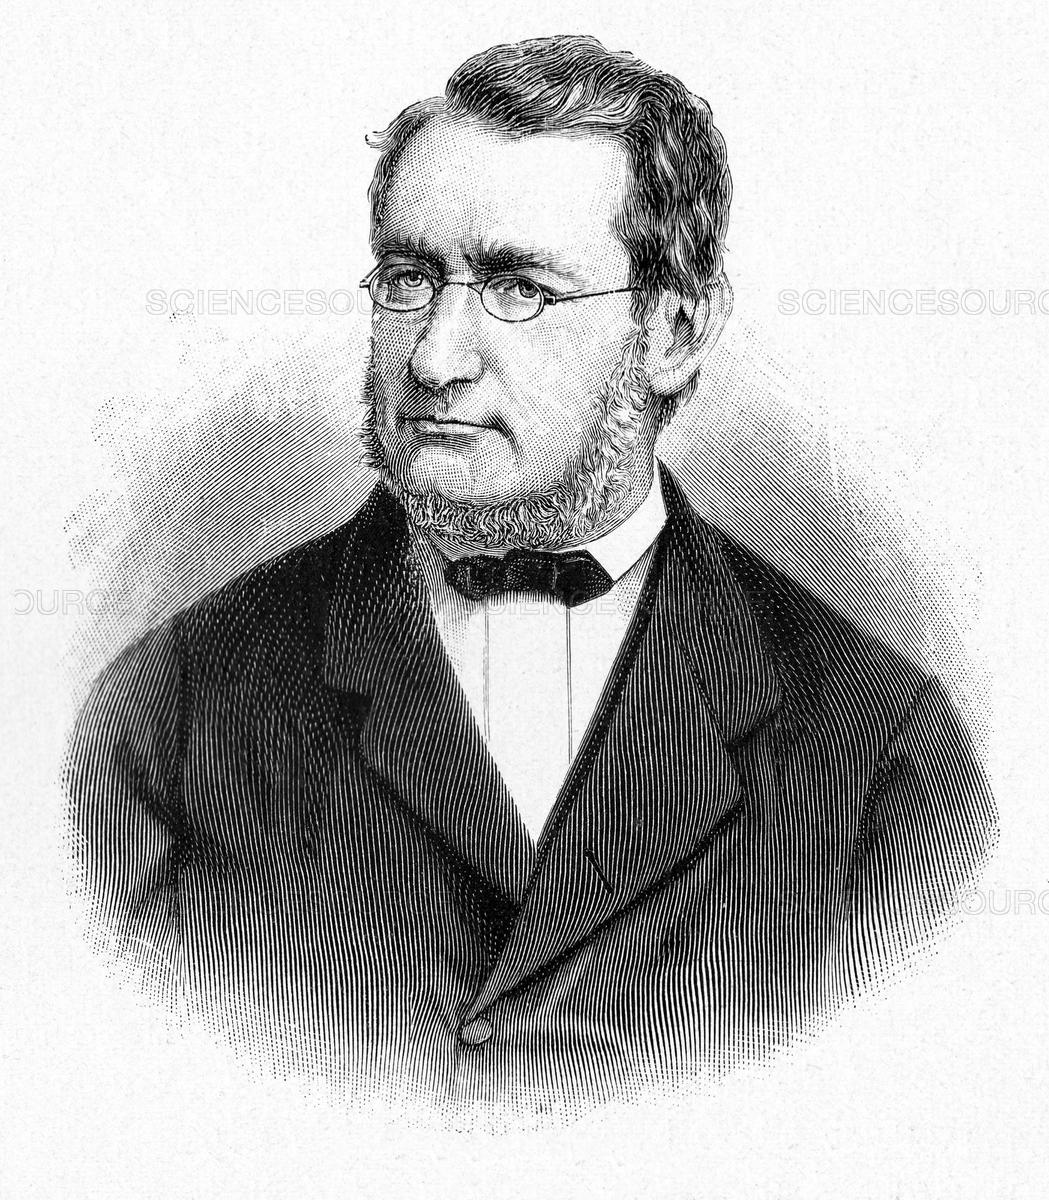
\includegraphics[width=0.25\linewidth]{sources/mayer} & 
			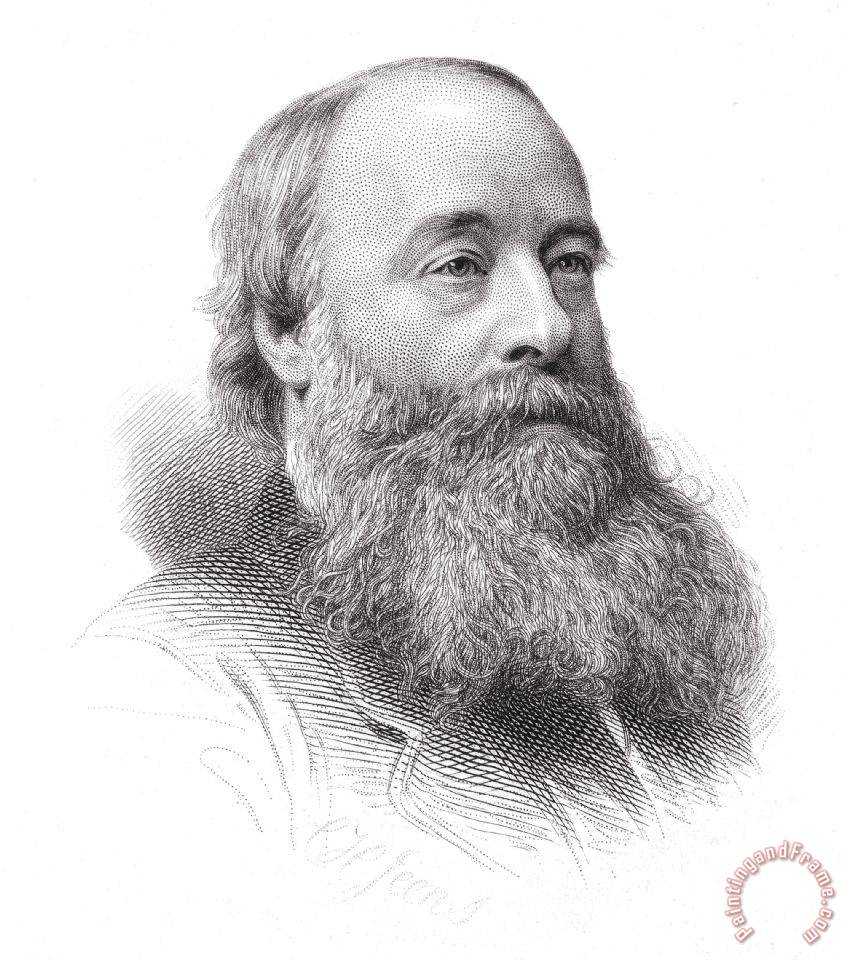
\includegraphics[width=0.25\linewidth]{sources/joule}\\
			Sadi Carnot & Julius von Mayer & James Joule	
		\end{tabular}
	\end{table}
	\begin{itemize}
		\item Thermodynamics is the study of energy transformations
		\item It was once thought that heat was a fluid
	\end{itemize}
\end{frame}

\begin{frame}{Introduction}
	\begin{columns}
		\begin{column}{0.5\textwidth}
			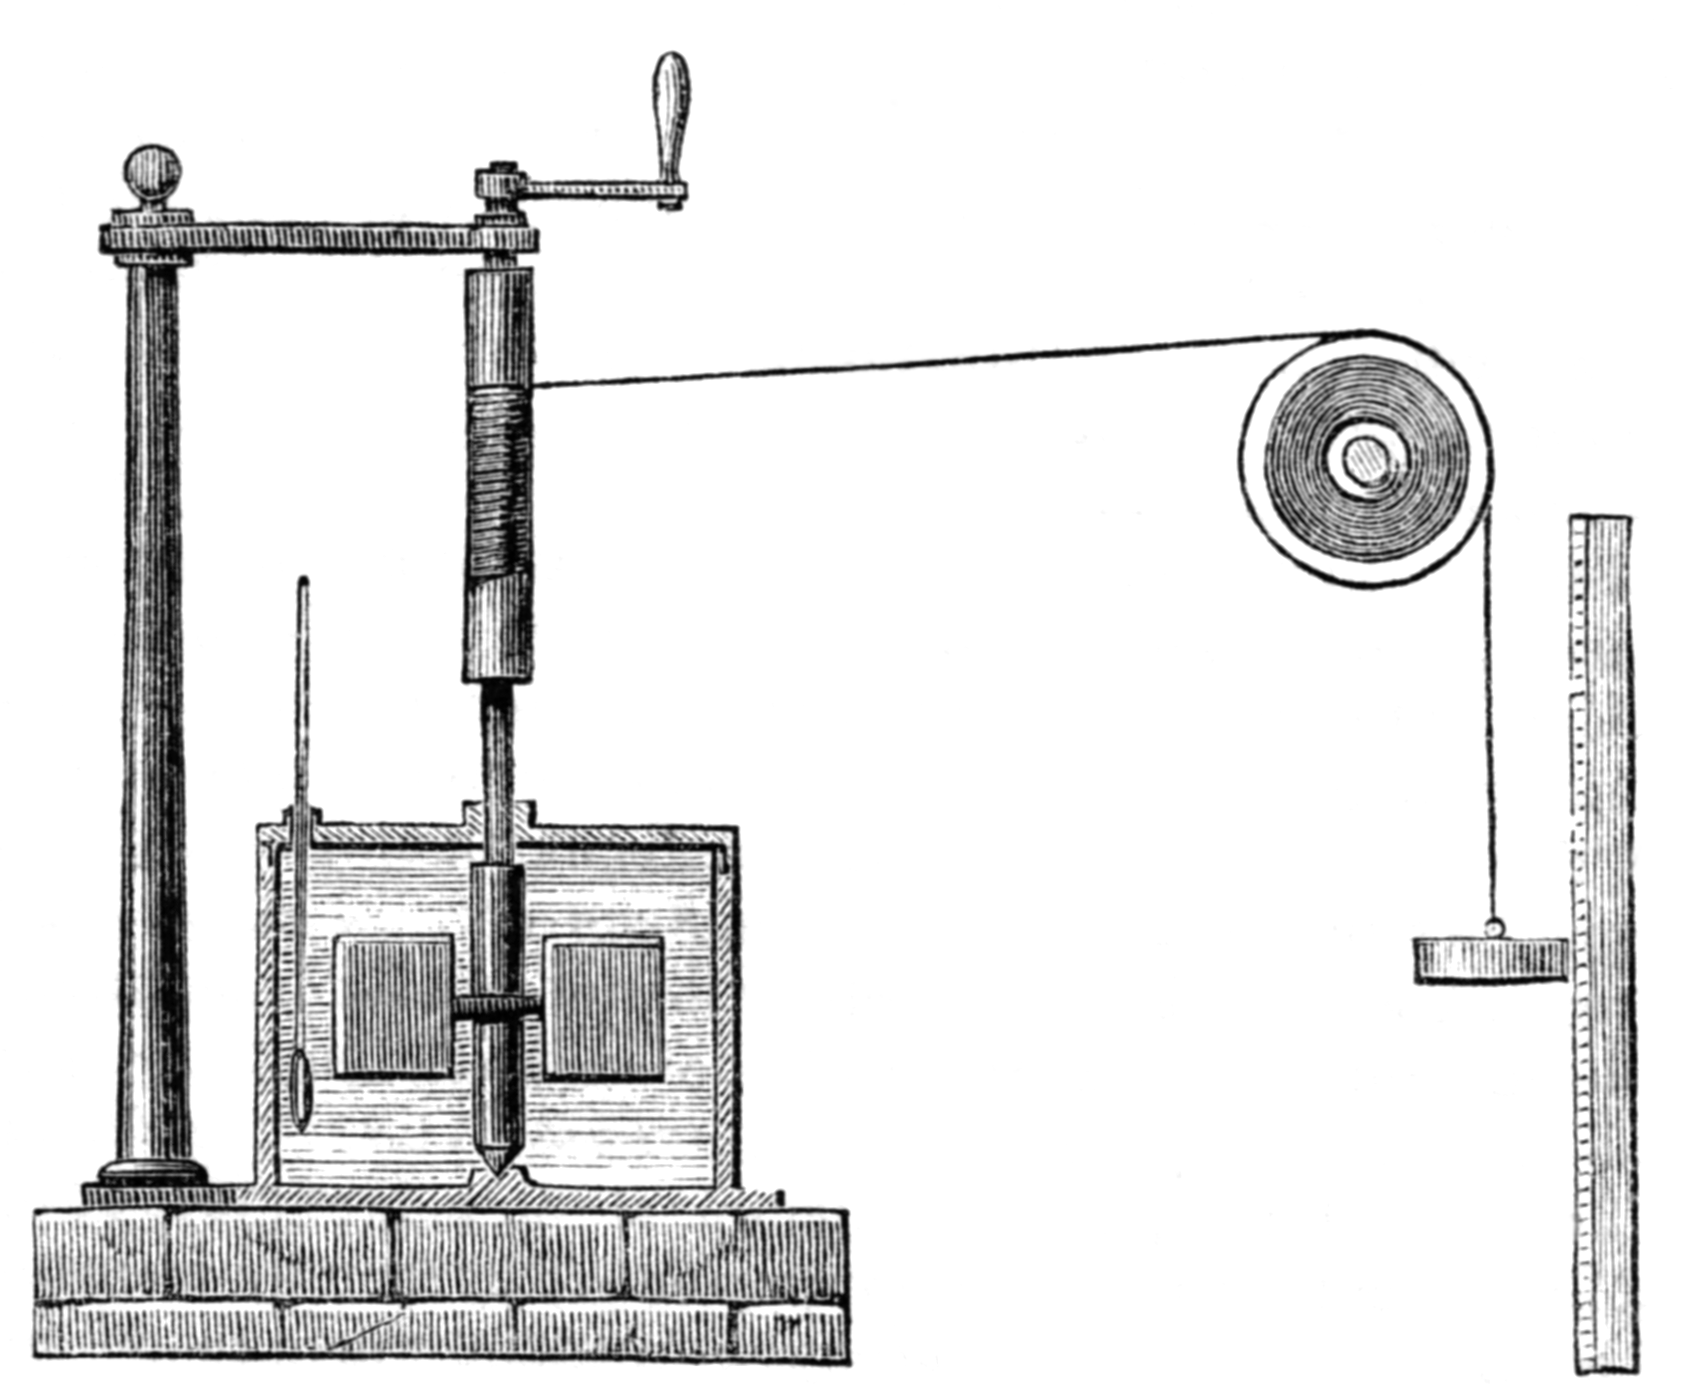
\includegraphics[width=\linewidth]{sources/joulesMachine}
		\end{column}
		\begin{column}{0.5\textwidth}
			\begin{itemize}
				\item $V = mgh$
				\item $T(V) = \dfrac{V}{m_{H_2O}C}$
			\end{itemize}
		\end{column}
	\end{columns}
\end{frame}

\begin{frame}{Introduction}
	\begin{itemize}
		\item How is heat measured?
		\item A Peltier element uses the Seebeck-Peltier effect to measure heat, and to transport it.
	\end{itemize}
	\begin{figure}[h]
		\centering
		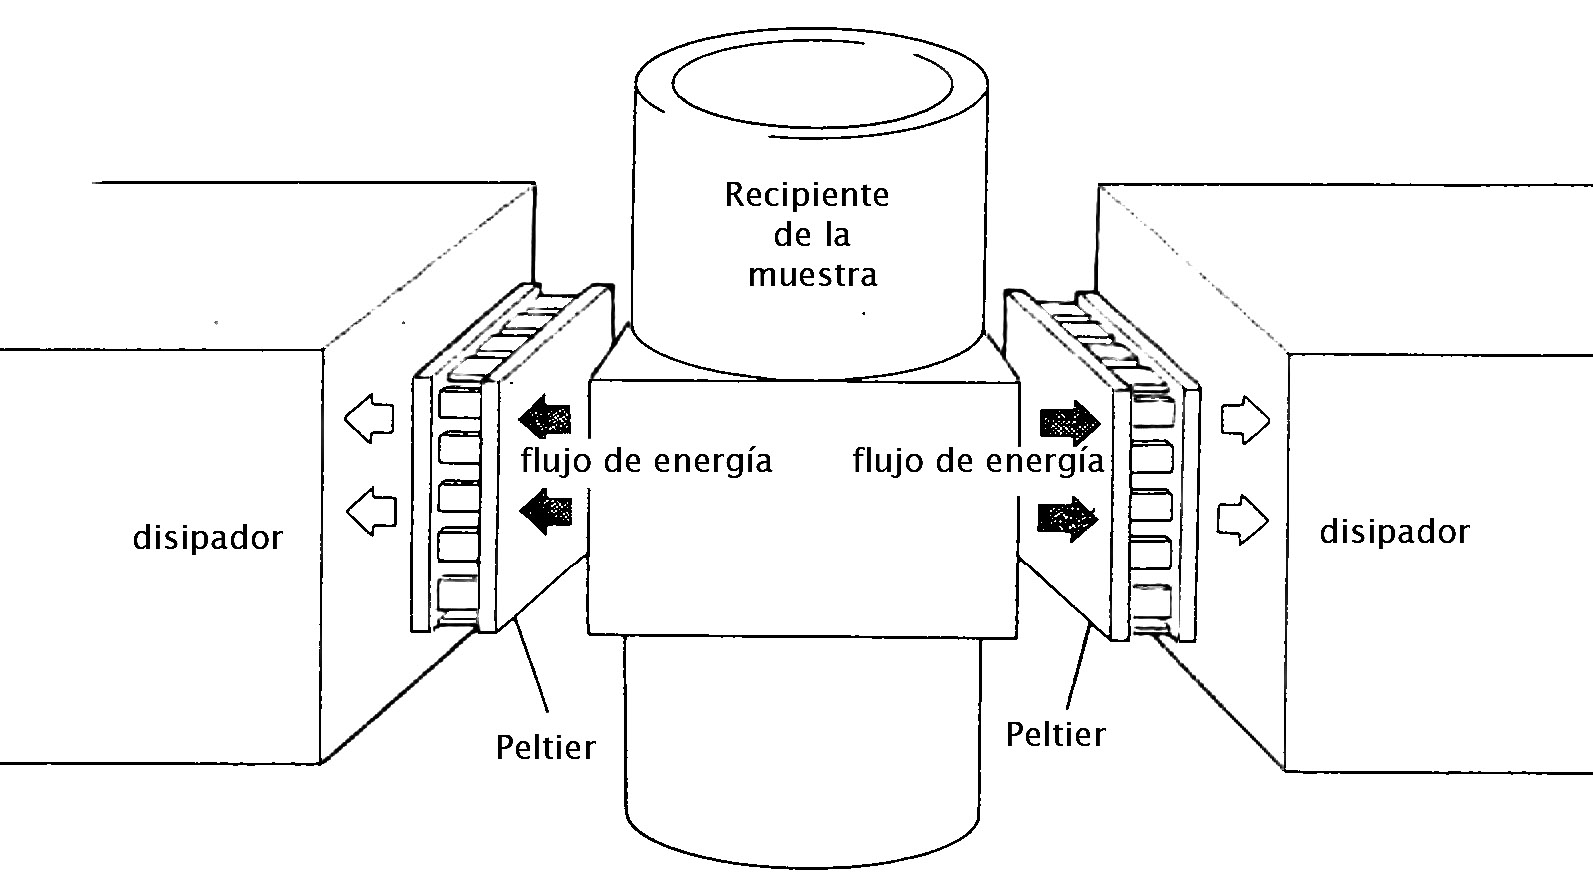
\includegraphics[width=0.8\linewidth]{sources/heatFlow}
	\end{figure}
	\begin{columns}
		\begin{column}{0.5\textwidth}
%			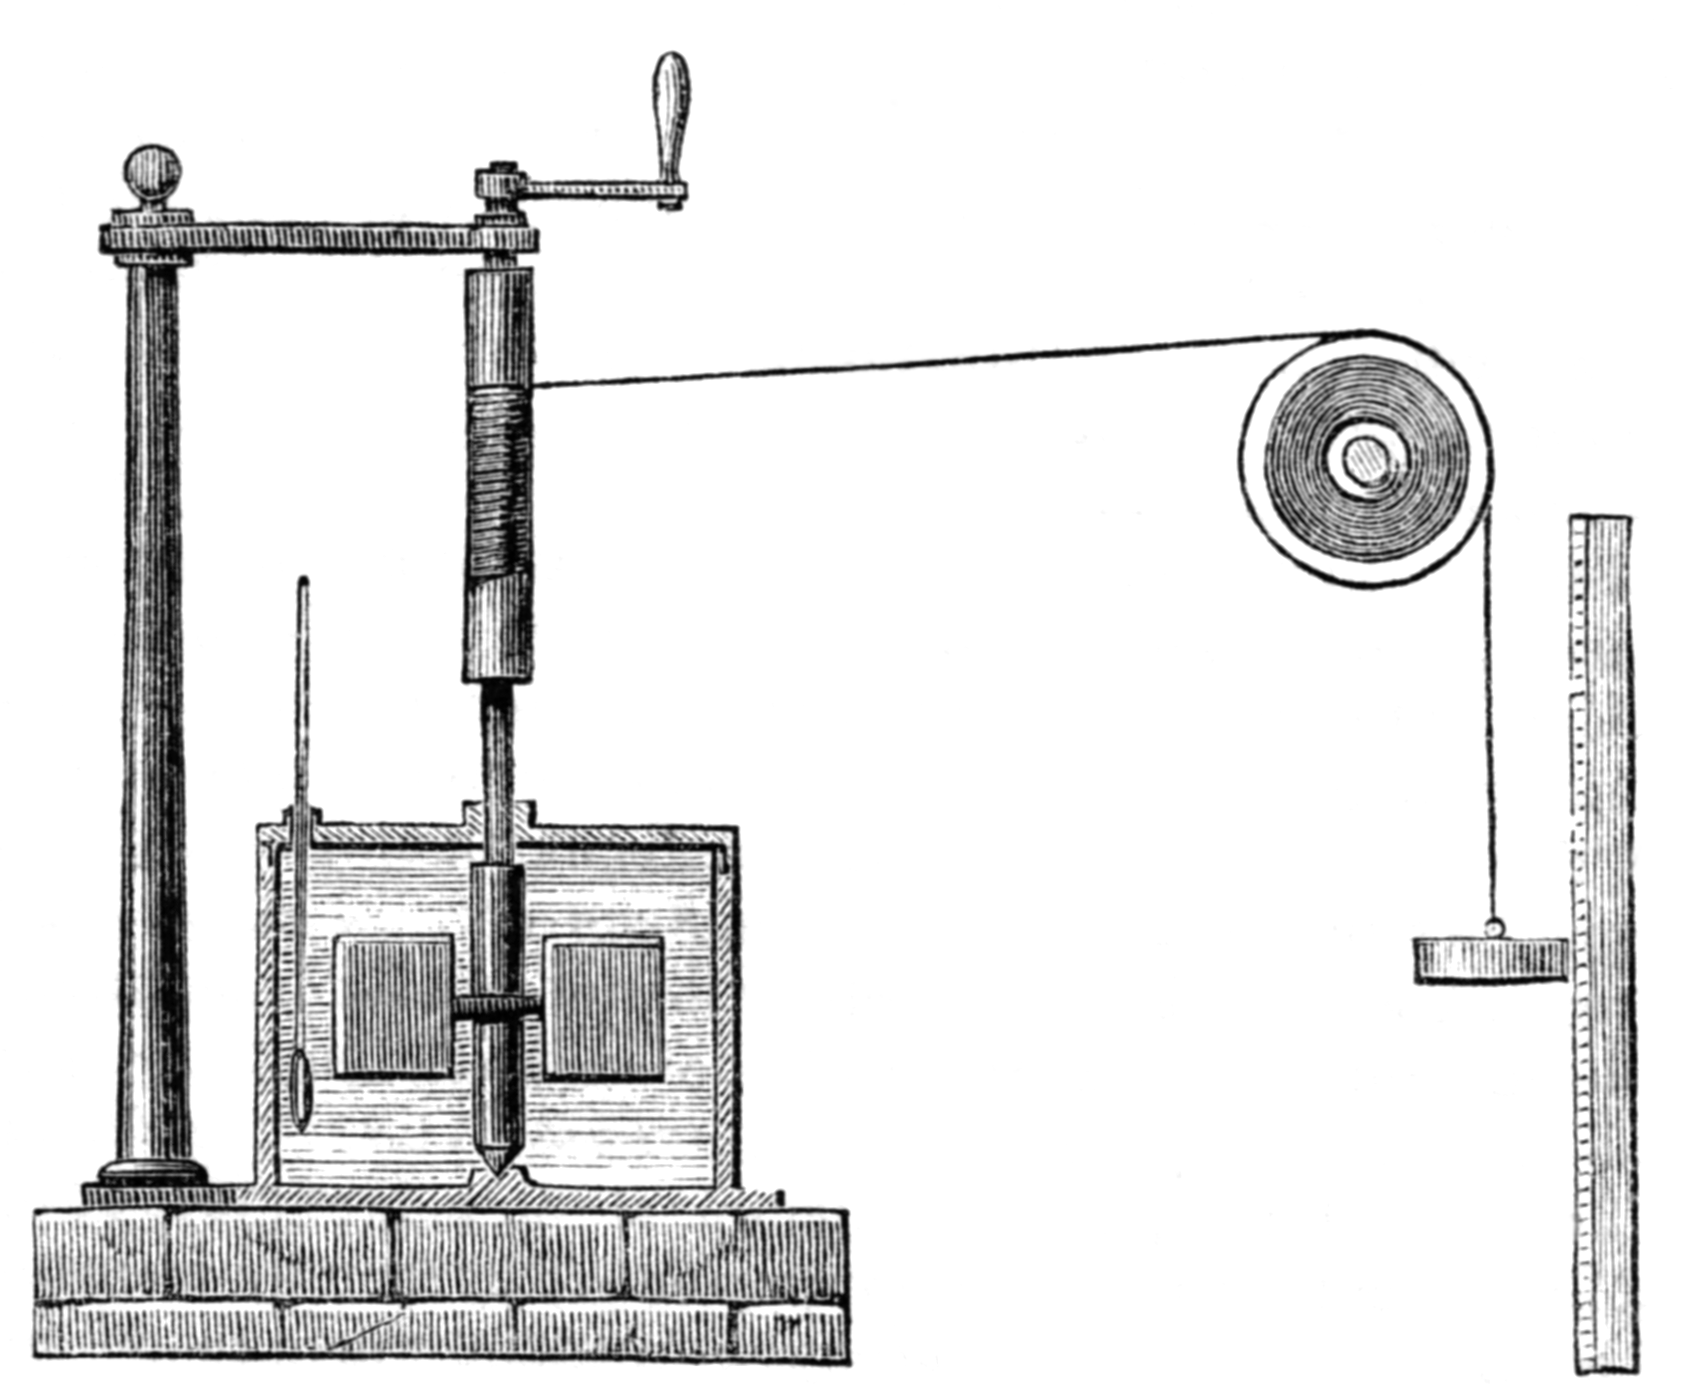
\includegraphics[width=\linewidth]{sources/joulesMachine}
			\begin{equation}
				V = -S\nabla T \propto Q
			\end{equation}
		\end{column}
		\begin{column}{0.5\textwidth}
			\begin{equation}
				Q = PIt
			\end{equation}
		\end{column}
	\end{columns}
\end{frame}

\section{Methodology}
\begin{frame}{Methodology}
	cries
\end{frame}

\section{Results and Discussion}
\begin{frame}{Results}
	peras
\end{frame}

\section{Conclusions}
\begin{frame}{Conclusions}
	hello
\end{frame}

\end{document}